\documentclass{bioinfo}
\usepackage{url}

\usepackage[british,english]{babel}
\usepackage{mathpazo}
\usepackage{color}
\definecolor{deepblue}{rgb}{0,0,0.5}
\definecolor{deepred}{rgb}{0.6,0,0}
\definecolor{deepgreen}{rgb}{0,0.5,0}
\definecolor{white}{rgb}{1,1,1}

\usepackage{listings}
\usepackage{setspace}

\definecolor{Code}{rgb}{0,0,0}
\definecolor{Decorators}{rgb}{0.5,0.2,0.2}
\definecolor{Numbers}{rgb}{0.5,0,0}
\definecolor{MatchingBrackets}{rgb}{0.25,0.5,0.5}
\definecolor{Keywords}{rgb}{0,0.6,0}
\definecolor{self}{rgb}{0,0,0}
\definecolor{Strings}{rgb}{0.6,0.,0}
\definecolor{Comments}{rgb}{0,0.63,1}
\definecolor{Backquotes}{rgb}{0,0,0}
\definecolor{Classname}{rgb}{0,0,0}
\definecolor{FunctionName}{rgb}{0,0,0}
\definecolor{Operators}{rgb}{0,0,0}
\definecolor{Background}{rgb}{1,1,1}
\definecolor{Modules}{rgb}{0,0,0.8}

\lstnewenvironment{python}[1][]{
\lstset{
%numbers=left,
numberstyle=\footnotesize,
numbersep=1em,
xleftmargin=0em,
framextopmargin=2em,
framexbottommargin=2em,
showspaces=false,
showtabs=false,
showstringspaces=false,
%frame=l,
tabsize=4,
% Basic
basicstyle=\ttfamily\footnotesize\setstretch{1},
backgroundcolor=\color{Background},
language=Python,
% Comments
commentstyle=\color{Comments}\slshape,
% Strings
stringstyle=\color{Strings},
morecomment=[s][\color{Strings}]{"""}{"""},
morecomment=[s][\color{Strings}]{'''}{'''},
% keywords
morekeywords={import,from,class,def,for,while,if,is,in,elif,else,not,and,or,print,break,continue,return,True,False,None,access,as,del,except,exec,finally,global,import,lambda,pass,print,raise,try,assert},
keywordstyle={\color{Keywords}\bfseries},
% additional keywords
morekeywords={[2]@parametric},
keywordstyle={[2]\color{Decorators}\slshape},
emph={self},
emphstyle={\color{self}\slshape},
%
}}{}


\usepackage[T1]{fontenc}
% \usepackage[latin9]{inputenc}
\usepackage{float}
\usepackage{amsmath}
\usepackage{graphicx}
\usepackage{setspace}
\usepackage{amssymb}
\usepackage{natbib}
\usepackage[title]{appendix}
\usepackage{siunitx}
\usepackage{chngcntr}
\usepackage{algorithmic}
\renewcommand{\algorithmicrequire}{\textbf{Input:}}
\renewcommand{\algorithmicensure}{\textbf{Output:}}

\usepackage{multirow}
\usepackage{rotating}
%\usepackage{xcolor}
\usepackage[pdfborder={0 0 0}]{hyperref}
%\usepackage{units}


\makeatletter
\newfloat{algorithm}{H}{loa}[section]
\floatname{algorithm}{Algorithm}
\counterwithout{algorithm}{algorithm}
\def\argmin{\mathop{\operator@font arg\,min}}
\def\argmax{\mathop{\operator@font arg\,max}}
\makeatother

\copyrightyear{}
\pubyear{}

\begin{document}
\firstpage{1}

\title[DIPY]{Dipy, a library for the analysis of diffusion MRI data}

\author[Garyfallidis, Brett, Amirbekian, Rokem, van der Walt, Descoteaux,
  Nimmo-Smith]{Eleftherios~Garyfallidis\,$^{1,2,*}$, Matthew~Brett\,$^{3}$,
  Bago~Amirbekian\,$^{4}$, Ariel~Rokem\,$^{5}$, Stefan~van der Walt\,$^{7}$,
  Maxime~Descoteaux\,$^{2}$, Ian~Nimmo-Smith\,$^{6}$ and Dipy~Contributors
  $^{8}$\footnote{to whom correspondence should be addressed. e-mail:
    garyfallidis@gmail.com}}

\address{\,$^{1}$University of Cambridge, Cambridge, UK\\
  \,$^{2}$University of Sherbrooke, Sherbrooke, CA\\
  \,$^{3}$University of California, Henry H. Wheeler, Jr. Brain Imaging Center, Berkeley, CA.\\
  \,$^{4}$University of California, San Francisco, CA, USA\\
  \,$^{5}$Stanford University, Stanford, CA, USA\\
  \,$^{6}$MRC Cognition and Brain Sciences Unit, Cambridge, UK\\
  \,$^{7}$Stellenbosch University, Stellenbosch, South Africa\\
  \,$^{8}$\texttt{http://dipy.org/developers.html}
  }

\history{}

\editor{}

\maketitle

\begin{abstract}
\noindent

Diffusion Imaging in Python (Dipy) is a free and open source software project
for the analysis of data from diffusion magnetic resonance imaging (dMRI)
experiments. DMRI is an application of MRI that can be used to measure the
micro-structure of the white matter in the human brain \emph{in vivo}. It
utilizes pulsed directionally oriented magnetic gradients to estimate diffusion
in different directions and locations in the brain non-invasively. Many methods
have been developed to model the local configuration of nerve fibers in the
white matter based on this information and to infer the trajectory of nerve
fascicles connecting different parts of the brain.

Dipy gathers implementations of many different methods, where they can be
easily understood and compared. Dipy aims to provide transparent
implementations for all the different steps of dMRI analysis with a uniform
API. We have implemented classical signal reconstruction techniques, such as
the diffusion tensor model and deterministic fiber tractography. In addition,
it implements cutting edge novel reconstruction techniques, such as constrained
spherical deconvolution and diffusion spectrum imaging with deconvolution, as
well as methods for probabilistic tracking and unique methods for tractography
clustering. Many additional utility functions, to calculate various statistics
of dMRI data, visualization functions, as well as file-handling routines exist
to assist in the development and use of novel techniques.

In contrast to many other scientific software projects, dipy is not being
developed by a single research group. Rather, it is an open project that
encourages contributions from any scientist/developer through the github Pull
Request mechanism and open discussions on github and on the project mailing
list. Consequently, dipy today has an international team of contributors,
spanning 6 different academic institutions in 4 countries and 3 continents,
which is still growing (http://dipy.org).

\section{Keywords:} Python, Diffusion MRI, Diffusion Tensor,
Spherical Deconvolution, Medical imaging, Free Open Source Software,
Deterministic tractography, Probabilistic tractography, Fiber tracking, Medical
Visualization.

\end{abstract}

\section{Introduction}

\emph{Diffusion MRI} (dMRI) \citep{stejskal-tanner:65, merboldt-hanicke-etal:85, lebihan-breton:85, taylor-bushell:85}
is an MRI technique \citep{callaghan:91} that provides information about the structure of neuronal
pathways found in the white matter and other body tissue with fiber-like
structure. DMRI acquires one or more $T_{2}$ reference images, and a collection
of diffusion-weighted images, in which $T_{2}$ signal is attenuated according
to the diffusivity of water along prescribed gradient directions
\citep{behrens-johansen-berg:09, jones:10}.

Because of its unique capability to characterize the micro-structure of neural
tissue, and the inferences that can be made using this information about
structural connectivity dMRI has had increasing popularity, with more than five
thousand papers published in 2012 only according to PubMed. This popularity is
also evident from the large number of software tools available for the analysis
of diffusion-weighted images. Many of these tools are written in C/C++: 3D
Slicer \citep{pieper:06}, AFNI \citep{cox-afni:12}, MITK
\citep{fritzsche-mitk:12}, BrainVoyager QX \citep{goebel-brainvoyager:12},
DTI-Query/Quench \citep{sherbondy:05}, FreeSurfer \citep{fischl-freesurfer:12},
FSL-FDT \citep{smith-fdt:04}, MedInria \citep{toussaint-souplet-etal:07},
MRtrix \citep{Tournier2012}, Diffusion Toolkit/Trackvis
\citep{wang-diffusion-toolkit:07}, FiberNavigator \citep{vaillancourt:11,
  chamberland:13}. Only a few are written in other languages, such as R:
TractoR \citep{ clayden-TractoR:11}, Java: Camino \citep{Cook2006} and Matlab:
ExploreDTI \citep{leemans-exploredti:09}, AFQ \citep{yeatman2012afq} and
others.

Dipy (\textit{Diffusion Imaging in Python}) \citep{garyfallidis2011dipy} is
the first collective effort to create an open-source diffusion MRI analysis
library using the Python language. Python is a general purpose, object-oriented
programming language which was designed with an emphasis on code readability.
This emphasis allows scientists who are not trained as software engineers to
understand the computational steps taken in analysis and extend the software in a
straight-forward manner. Being an interpreted language, Python does not require
additional compilation, linking, etc. and so installation of software written
in Python is relatively easy. Taken together, these properties of the language
are powerful assets for the design of the next generation of medical imaging
analysis tools. In the past we found that many researchers were using available
tools without understanding the underlying details, often because the details
were hidden from the users. Dipy tackles this problem by being free, open
source (BSD license), simple and well documented. In addition, the recent
explosion of Python users, the many Python tools for scientific computing
\citep{perez_python:11}, \citep{mckinney_python:12}, \citep{perez_ipython:07}
and the recent stack of neuroimaging\footnote{\url{http://nipy.org}} modules
make Dipy a useful addition for those who prefer Python as their favorite
language.
Dipy takes advantage of the growing ecosystem of tools written for scientific
computing in Python. It is built on top of production-ready high-performance
Python libraries. Primarily, Dipy depends on
Numpy\footnote{\url{http://numpy.org}}. The core structure of this library is
an implementation of an Array \citep{van_numpy:11} class. Numpy arrays are used
for representation of numerical data in Python and enable efficient
implementation of numerical computations, such as vectorized computations,
avoiding copying data in memory, and minimizing operations. Numpy is also used
for matrix, tensor and linear algebra operations.  Dipy further depends on
Scipy\footnote{\url{http://scipy.org}} for nonlinear optimization and other
volumetric operations. Cython\footnote{\url{http://cython.org}} is used in rare
cases when both standard Python and Numpy/Scipy are not efficient enough for
the task at hand. Cython interprets Python code into plain C performance by
adding static type declarations. The last absolute dependency for Dipy is
Nibabel\footnote{\url{http://nipy.org/nibabel}} which is used for loading and
saving medical imaging file formats.

Optional dependencies, that are not required for analysis, are used for
visualization of diffusion data and the results of
analysis. Matplotlib\footnote{\url{http://matplotlib.org}} is used for 2D and
3D plotting. In addition, Python-VTK\footnote{\url{http://vtk.org}} is used for
more advanced 3D interactive visualization. Furthermore, we recommend using
IPython\footnote{\url{http://ipython.org}} the interactive Python shell for
calling and debugging our scripts.

In the following sections, we will explain the philosophy and main design
concepts behind Dipy. We will also give examples which cover different parts of
the diffusion MR analysis pipeline from the local voxel reconstruction of
orientation distribution functions to streamline generation and visualization.

\section{Philosophy and Mission}

Mission: The purpose of Dipy is to make it easier to do better diffusion MR
imaging research. We aim to build software that is clearly written, clearly
explained, well tested, a good fit for the underlying ideas and a natural home
for collaboration.

Dipy is a true international project where anyone from anywhere in the world
is welcome to contribute as long as they agree with the project's mission
statement. In order to be faithful to this mission, all contributors are
required to follow certain policies. For example, if a scientist makes a new
discovery---even one of substantial importance---and wants to share the code,
it will not be integrated in the main project without extended testing as well
as code reviews from at least two members of the team.  Such principles
aim to help the Dipy code-base preserve its quality while growing.

Through this work ethic Dipy has attracted an international and
multi-departmental team of highly skilled contributors from different levels
of education (Master students, PhD students, Post-Docs and Professors)
spanning the fields of Computer Science, Medicine, Applied Mathematics,
Biomedical Engineering and Psychology.


\section{Terminology}

As in many other fields of science, dMRI is a field that uses specific
terminology to describe the constructs of the measurement, as well as to
describe the interpretation of the results of the analysis. We rely on a recent
paper \citep{Cote2013tractometer}, that has proposed specific terminology for
describing different constructs of the dMRI field. In this section we will
describe constructs of the measurement, as well as constructs used to interpret
the results of the analysis. We will use this terminology to explain the
analysis code and interpretation of data in subsequent sections.

The measurement of dMRI data relies on the application of a pulsed magnetic
gradient and the degree of sensitization to diffusion depends on a number of
parameters, including the duration of the gradient, time that elapses between
pulses of the gradient and the gradient amplitude. These parameters are
together summarized in what is referred to as the "b-value".  As described
above, the measurement is conducted in several different directions and these
are encoded in so-called "b-vectors". These are unit vectors that describe the
direction relative to the scanner coordinate frame in which the gradients are
applied. Different algorithms are used to determine the placement of these b-
vectors (e.g. \citep{jones-etal:99}).

While we are ultimately interested in the identification of the trajectories of
bundles of axons, which are the long fiber-like part of a nerve cell along
which electrical impulses are conducted from cell to cell (and whose size is on
the $\mu$m scale), the measurement is conducted on a much larger
scale. Typically, the measurement is conducted in a grid of "voxels" of
approximately 2x2x2 mm. We are therefore limited to describe the trajectories
of "fascicles" of nerves. One of the major achievements of this field is that
it is now possible to reliably and accurately identify major fascicles in
individual experimental participants or patients. These major fascicles are
also known as "tracts". This is a term taken from neuroanatomy and describes a
group of neuronal axons within the central nervous system (mm scale).

For the purpose of interpretation of these data, a "fiber" can be any long and
thin structure. Hence, fiber tracking is a general term that can be used in any
field that reconstructs fibrous structures, such as hair fibers, celery fibers,
muscle fibers, prostate fibers, brain fibers, etc. "Fiber bundles" denote
groups of fibers usually with an anatomical or functional meaning. These can be
major tracts in the brain, such as the arcuate fasciculus, which connects parts
of the posterior temporal lobe with the frontal lobe, the fornix, which
connects the medial temporal lobe with sub-cortical structures, such as the
hypothalamus and amygdala, etc. A fiber bundle for the area of brain anatomy is
synonymous to a tract, also often called fiber tract. The term tract can be
misleading when talking for example about the corticospinal tract, because the
corticospinal tract is in fact not a single tract but a group of tracts
(including corticobulbar projections, the pyramidal tract, etc.).

Tractography is the computational process through which the fibers are detected
and delineated. Tractography relies on the assumption that diffusion of water,
as reflected in the dMRI measurement, occurs more freely along the axis of an
axon, than across the membranes of the axon. Tractography is therefore usually
done by finding the directions of diffusion in each voxel (see
\ref{reconstruction}) and stepping through the brain volume along the
directions of large diffusion estimated in each location. This process
generates so-called streamlines, which imaginary lines that approximate the
underlying fiber. Streamlines are also sometimes referred to as "tracks". These
are not to be confused with tracts: While a tract is a physical object, a track
is a computational construct that only approximates the underlying fascicle or
bundle of fibers. Confusingly enough "streamline bundles", or simply "bundles"
are often used to refer to a group of streamlines with similar shape and
spatial characteristics (see \ref{quickbundles}). These do not necessarily 
correspond to individual physical fiber bundles but are instead computational 
constructs that approximate the underlying anatomy.

\section{General design aspects}

Dipy is built on the Scipy tool stack, which includes packages such as
Numpy (numerical arrays and array computation), Scipy
(scientific libraries, e.g. optimization, triangulation, special functions,
and more) and Cython (an optimized Python to C compiler, used to achieve
native performance).  Furthermore, it integrates into the Nipy (neuroimaging
in Python) eco-system of software (see Fig.~\ref{Fig:module_structure}).

Dipy's API is designed with the aim to be intuitive, simple to use, and well
documented.  This allows researchers to rapidly construct even complex
computational experiments while retaining code readability.  In addition,
since the code is entirely free and open, Dipy is ideally suited to facilitate
reproducible research.

Like many modern open source projects, Dipy is hosted on GitHub---an online
version of the Git revision control system. Changes are made via a Pull
Request (PR) mechanism, whereby submissions can be proposed, discussed and
iterated upon before being included finally. The discussions also allow for
line-by-line comments to be made by any interested developer.

To assist developers, Dipy uses the Travis continuous integration system.  Any
time a new PR is proposed, Travis commissions a new virtual machine, installs
the necessary dependencies, builds a clean copy of Dipy, and runs Dipy's
test suite against the new changes.  Only if no failures are reported will the
new code be considered for inclusion.  Dipy also follows a test-driven
development philosophy, whereby all code should be accompanied by a suite of
tests to exercize all corner cases.

For documentation, Dipy utilizes Sphinx, the same system employed by the main
Python project.  Sphinx takes plain-text ReStructuredText as input and
converts it to either HTML, LaTeX or PDF formats.  API documentation is
extracted directly from the docstrings in the source code, so that it is never
outdated.

Dipy's main sub-modules (see Fig.~\ref{Fig:module_structure}) are \emph{core}, 
\emph{reconst, tracking, viz, io, align, data, sims} and \emph{segment}. 
\emph{Core} contains general functions that can be used in any other sub-module. 
\emph{Reconst} contains classes for voxel-based reconstruction. \emph{Tracking} 
holds classes for fiber tracking and streamline processing. \emph{Viz} is used
 for 3D vizualization and interaction. \emph{Io} offers input/output utilities
when they are not available in Nibabel. \emph{Align} provides tools for 
alignment and reslicing of volumes or streamlines. \emph{Sims} is focused on 
creating synthetic simulations. \emph{Data} is used for downloading public 
datasets. \emph{Segment} concentrates on segmentation of images and clustering
of streamlines.

\begin{figure}
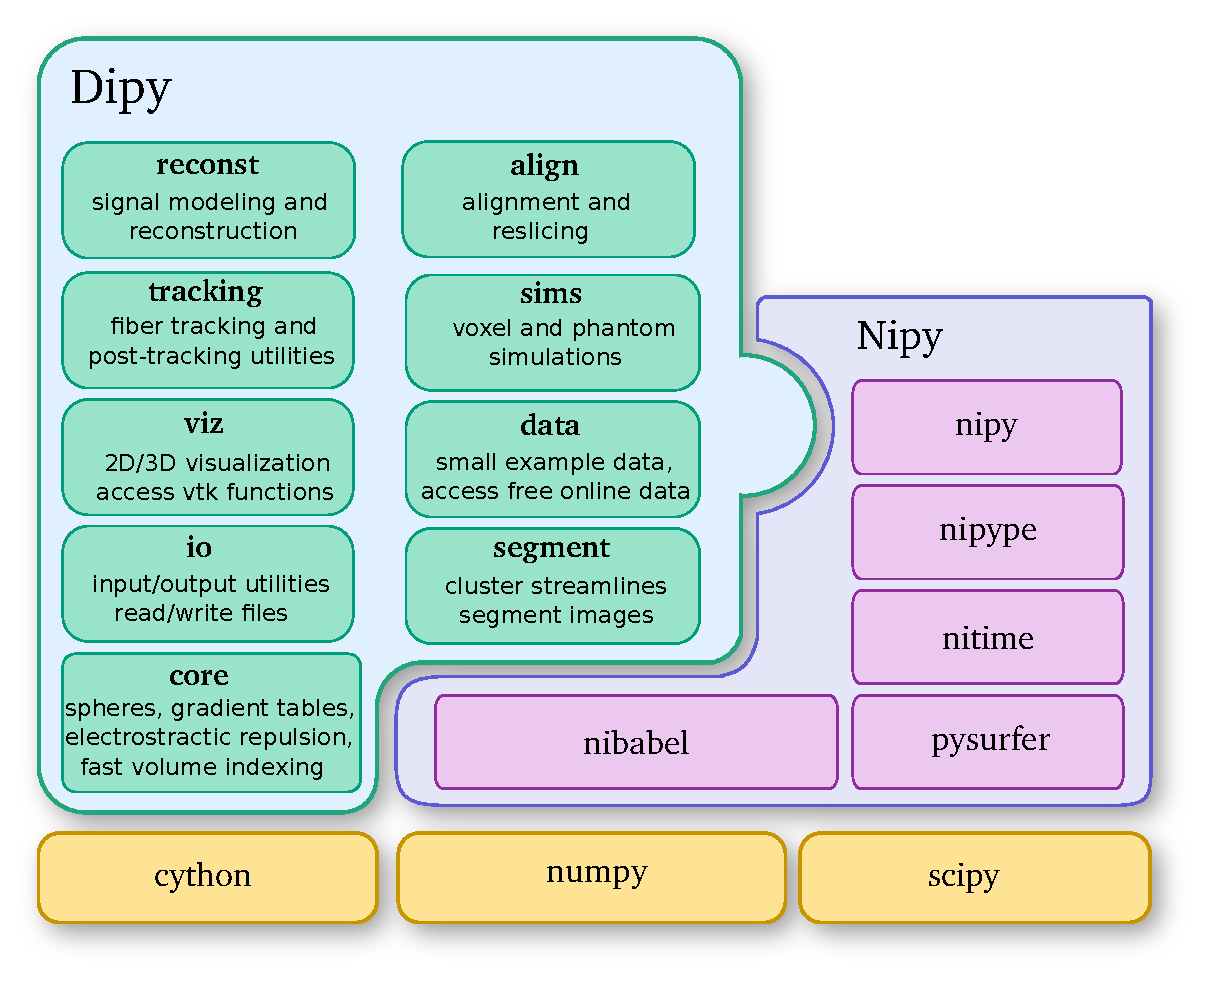
\includegraphics[scale=0.42]{Figures/module_structure2.eps}
\centering{}
\caption{Dipy is one of the main projects of the Nipy community and depends strongly
on Numpy, Scipy and Cython. This diagram further shows the major Dipy sub-modules.\label{Fig:module_structure}}
\end{figure}

In this paper we will use code listings to illustrate the use of Dipy. For 
example, the following code snippet shows how to find your current version of 
Dipy.
\begin{python}
import dipy
dipy.__version__
'0.7.0.dev'
\end{python}

\section{Preprocessing}\label{preprocessing}

\subsection{Load/Save data}\label{loadsave}
The most basic operation that we do in Neuroimaging is to load some data from
the disk which are generated from an MRI scanner. Surprisingly this is often a
difficult task as different scanners and software read/write the data in
different ways. Nibabel, a library for reading medical imaging formats, is
coming here to the rescue supporting ANALYZE (plain, SPM99, SPM2), GIFTI,
NIfTI1, MINC, MGH, ECAT, PAR/REC, Freesurfer (geometry, morphometry files) and
with a growing support for DICOM.

The most common file format used in dMRI is the NIfTI1. Assuming that we have a
file with our 4D raw diffusion data we can load it in the following way:
\begin{python}
fimg = "raw.nii.gz"
import nibabel as nib
img = nib.load(fimg)
\end{python}
Where \texttt{fimg} holds the filename for the 4D NIfTI1 file, \texttt{nib} is
a shortcut for the Nibabel module, \texttt{img} is an object that Nibabel
creates which contains all the information from the file e.g. the header, the
data and the affine. We can obtain all these using \texttt{getter} methods:
\begin{python}
data = img.get_data()
affine = img.get_affine()
header = img.get_header()
voxel_size = header.get_zooms()[:3]
\end{python}
Here \texttt{data} is a Numpy array which contains the actual 4D image (a
collection of 3D volumes). Using \texttt{data.shape} we can obtain the
dimensions of the image. In this example the dimensions are (81, 106, 76,
160). The first three dimensions contain the size of the volume and the last
dimension has the information for the different diffusion gradients. The
variable \texttt{affine} provides a $4\times4$ matrix which contains the
transformation matrix which maps voxel image coordinates to world mm
coordinates. This matrix can be useful when registering, saving or visualizing
images. The \texttt{voxel\_size} is a tuple with 3 values. In this example the
\texttt{voxel\_size} is (2, 2, 2) i.e. $2~mm^3$.

Supposing that we want to extract and save from the 4D data only the first volume which usually is the one without any diffusion gradients. This volume is also known as the \texttt{S0}. We can do that very easily using the following code.
\begin{python}
S0 = data[:, :, :, 0]
img2 = nib.Nifti1Image(S0, affine)
nib.save(img2, "S0.nii.gz")
\end{python}
As we said previously \texttt{data} is a Numpy array. Numpy arrays provide
simple ways to extract information from N-dimensional datasets, an operation
known as slicing. For example, \texttt{data[10:20, 10:20, 10:20, 30:50]}
returns a new sub-array with \texttt{shape} (10, 10, 10, 20). When a single
column (:) is used that means that all points in this dimension are used. The
only delicate point here is that in order to save this new array we will need
to update the affine. This is possible in the following way:
\begin{python}
import numpy as np
sub_data = data[10:20, 10:20, 10:20, 30:50]
sub_affine = affine.copy()
sub_affine[:3, 3] += np.array([10, 10, 10])
sub_img = Nifti1Image(sub_data, sub_affine)
nib.save(sub_img, "sub_data.nii.gz")
\end{python}

\subsection{Background removal}
In order to remove the background and keep only the parts that are in the brain
we can use a function called \texttt{median\_otsu}.
\begin{python}
from dipy.segment.mask import medotsu
mask, S0_mask = medotsu(data[:, :, :, 0])
\end{python}
\texttt{median\_otsu} uses first a median filter to smooth the \texttt{S0} and 
then otsu, an automated histogram method [REF] to separate the brain
(foreground) from its background. It returns two arrays, the \texttt{mask}, a
3D array with 1s at the foreground and 0s in the background and the masked
\texttt{S0}, \texttt{S0\_mask} a 3D array whith the actual \texttt{S0} values in
the foreground and 0s in the background.

\subsection{Gradient Table}\label{gtab}
The b-value $b$ or \emph{diffusion weighting} is a function of the amplitude,
duration, temporal spacing and timing parameters of the specific paradigm. In
the case of the classical Stejskal-Tanner pulsed gradient spin-echo (PGSE)
sequence, at the time of readout
$b=\gamma^{2}G^{2}\delta^{2}\left(\Delta-\delta/3 \right)$, where $\gamma$ is
the gyromagnetic ratio, $\delta$ denotes the pulse width, $G$ is the gradient
amplitude and $\Delta$ the centre to centre spacing. $\gamma$ is a constant
which depends on the nucleus, but we can change the other three parameters and
in that way control the b-value. By changing the b-value along different
gradient directions the MR physists can alternate the quality and duration of
the dMRI experiment. The gradient unit directions are often referred as
b-vectors. Both b-values and b-vectors are absolutely necessary knowledge for
analysing diffusion data and can be usually read from one or two different
files. Here is an example:
\begin{python}
fbval = "raw.bval"
fbvec = "raw.bvec"
from dipy.io import read_bvals_bvecs
bvals, bvecs = read_bvals_bvecs(fbval, fbvec)
\end{python}
These parameters are stored in a utility class, created by the \texttt{gradient\_table} function:
\begin{python}
from dipy.core.gradients import gradient_table
gtab = gradient_table(bvals, bvecs)
\end{python}
Here, \texttt{gtab} is an instance of a \texttt{GradientTable} object. This
object makes sure that the b-values and b-vectors will come out in a form that
Dipy knows how to use. For example, the \texttt{shape} of
\texttt{gtab.bvals} and \texttt{gtabl.bvecs} should always return $N$ and
$N\times3$ respectively, where N is equal to the size of the last dimension of
\texttt{data}. Often, it is useful to know the number and position of b-values
with value 0 (b0s), an utility method is provided for this purpose with
\texttt{gtab.b0s\_mask}.

The \texttt{GradientTable} object can be used not only to store b-values and
b-vectors but also other acquisition parameters like TR, TE, $\delta$ and
$\Delta$. Therefore, it is an abstract representation of the acquisition
specific parameters.

\section{Reconstruction}\label{reconstruction}

In diffusion MRI, the motion of water molecules is probed in a spatial- and
direction-specific manner. That is, in every spatial location in the brain
(typically sampled in voxels each covering a volume of approximately
$2\times2\times2$ mm), the diffusion in several different directions is probed
through the application of directional magnetic gradients. This motion takes
place at a microscopic level, therefore, if we want to describe how the
molecules diffuse we have to study this phenomenon from a statistical
point of view. When a molecule is at position $\mathbf{x}_{0}$, we cannot read
exactly where it will be after time $t$, we can only model a distribution of
possible locations i.e. a probability displacement distribution. This is also
known as the diffusion propagator $P$. This motion is described by the
propagator $P(\mathbf{x};\mathbf{x}_{0},t)$ which defines the probability of
being in $\mathbf{x}$ after a time $t$, starting at $\mathbf{x}_{0}$.  Stejskal
and Tanner \citep{stejskal-tanner:65} showed that the spin echo magnitude
$S(\mathbf{q},t)$ from a pulsed gradient spin echo (PGSE) experiment is
directly related to the diffusion propagator by the following (inverse) Fourier
relation
\begin{equation}
S(\mathbf{q},t)=S_{0}\int P(\mathbf{r},t)e^{i\mathbf{q}\cdot\mathbf{r}}d\mathbf{r}\label{eq:fourier}
\end{equation}
\noindent where $S_{0}$ is the signal in the absence of the applied magnetic
diffusion gradient $\mathbf{g}$, $\mathbf{r}$ is the relative spin displacement
$\mathbf{x}-\mathbf{x}_{0}$ at diffusion time $t$ and $\mathbf{q}$ is the spin
displacement wave vector. $\mathbf{q}$ is parallel with the applied magnetic
gradient $\mathbf{g}$ which in turn are directly related with the b-vectors
discussed in section \ref{gtab}.  In theory, if we apply the Fourier
transform in eq.~\ref{eq:fourier} we can get back a 3D PDF (the diffusion
propagator) for every voxel. In practice, unfeasibly long acquisition time is
required and perfect experimental conditions. Therefore, a discrete method
called Diffusion Spectrum Imaging(DSI) has been used (see section \ref{dsi}).
Nonetheless DSI still needs long acquisitions. An alternative is to work on
reconstructing only a spherical projection of the 3D PDF. This often called the
diffusion orientation distribution function (dODF) or simply ODF. Another
alternative is to make assumptions about the distribution of the PDF. In this
later category belongs the most popular imaging method in dMRI: Diffusion
Tensor Imaging (DTI).

\subsection{Diffusion Tensor Imaging}\label{dti}

Often people assume that DTI and dMRI are synonymous. This is not correct. In
DTI there is a crucial assumption that the propagator is described only by a 3D
Gaussian distribution. With this assumption from eq.~\ref{eq:fourier} we can
write
\begin{equation}
P(\mathbf{r},t)=\frac{1}{\sqrt{4\pi t^{3}\mid\mathbf{D}\mid}}exp(-\frac{\mathbf{r}^{T}\mathbf{D}^{-1}\mathbf{r}}{4t})
\end{equation}
\noindent where $\mathbf{D}$ is known as the diffusion tensor. This tensor is a
$3x3$ positive definite symmetric matrix that can be completely described by a
centered ellipsoid with 3 principal axes and associated eigenvalues
$\lambda_{1},\lambda_{2},\lambda_{3}$.

DTI was first proposed by Basser and colleagues
\citep{basser-mattiello-etal:94} and has since been very influential in
demonstrating the utility of dMRI in characterizing the micro-structure of
white matter tissue. The model relies on the assumption that diffusion is a
Gaussian process. Using this assumption the dODF can be modeled with 6
parameters, describing the variance and covariance of the Gaussian diffusion
along the three primary axes. From these parameters, several useful measures
can be derived: the primary diffusion direction is the primary eigen-value of
the tensor, $\lambda_{1}$ and it is the direction in which variance in the
diffusion distribution is largest. In some places in the brain (e.g. in the
corpus callosum, the large fiber bundle in the center of the brain that
connects the two hemispheres) this corresponds to the direction of the white
matter fibers in the voxel and can be used for tracking
\citep{conturo-lori-etal:99, Mori1999, Basser2000}. Other univariate measures
are estimated from the parameters of the model to assess the biophysical
properties of the underlying tissue. The diffusivity along the primary
direction (referred to as axial diffusivity, or AD) and along other directions
(radial diffusivity, or RD), as well as the mean diffusivity (MD) are thought
to index proportions of extra-cellular and intra-cellular water within the
voxel. For example, MD is commonly used in the diagnosis of acute ischemic
stroke, because these types of brain injury are characterized by cell-body
swelling. The reduction in extracellular water fraction results in a decrease
in MD in the affected regions \citep{Maas2005}.

The fractional anistropy (FA) is a normalized measure of the variation in
diffusivity between different directions and was originally thought to index
the organization of the tissue within the voxel \citep{Basser1996}. Later
studies in animal models demonstrated that FA decreases when demyelination
occurs \citep{Song2002}, because of increases in radial diffusivity. These
studies showed that in the white matter degree of myelination is an important
factor in limiting diffusion of water across cellular compartments. In
addition, tissue density affects both the radial and the axial diffusivity, and
loss of nerve fiber tissue also results in a decrease in FA \citep{Beaulieu1996,
  Beaulieu2002}. As a consequence of these studies, researchers now routinely
refer to FA as a measure of "tissue integrity". However, we strongly warn
against this usage, because it is easy to show that though the density of the
tissue and the density of the myelin wrapping the axons in the voxel may affect
both MD and FA, changes in other factors, such as the distribution of
directions of crossing of fiber populations throught the voxel may also affect
these measures \citep{Basser1996,wandell-yeatman:13}. Therefore, interpretation
of group differences in FA, or longitudinal changes in FA over time should be
carefully handled and compared to the results from other modeling techniques,
that better account for the distribution of fiber orientations in the voxel
(see below).

That said, the use of DT-based univariate statistics is very popular among
users of dMRI and also quite useful. That is, variance in a variety of
behavioral \citep{Ben-Shachar2007} and clinical \citep{Thomason2011} measures
can be predicted based, suggesting that they are reporting on meaningful and
impactful variability in brain structure.

Fitting the tensor model and computing univariate statistics from it in Dipy is
straightforward. In the following example, we show how the tensor model is fit
to data and how univariate measures can be computed.

First, \texttt{data}, \texttt{mask} and \texttt{gtab} are created as we saw in
section \ref{preprocessing}. Next, we can import the diffusion tensor model class
and initialize a \texttt{TensorModel} class instance with the name
\texttt{ten\_model}:
\begin{python}
from dipy.reconst.dti import TensorModel
ten_model = TensorModel(gtab)
\end{python}
Note that at this point in the code no data analysis has occurred yet. Since
the analysis of every voxel in the brain will rely on similar infra-structure,
the \texttt{TensorModel} class instance only sets up the skeleton for the
analysis. This same skeleton will be reused for each one of the voxels in the
data here, but can also be reused for other data in a similar fashion.  Next,
we pass the data to the fit method of the \texttt{tensor\_model}. This returns
a \texttt{TensorFit} class instance which relates to the specific data and
mask:
\begin{python}
ten_fit = ten.fit(data, mask)
\end{python}
The advantage of this separation of the model and the fit is that we can fit
many different data with the same initialization parameters without duplicating
code. Once a fit has been conducted, we can compute a variety of derived
univariate measures, such as the fractional anisotropy (FA) [REF]:
\begin{python}
from dipy.reconst.dti import fractional_anisotropy
fa = fractional_anisotropy(ten_fit.evals)
\end{python}
It is common to represent the primary diffusion direction using an RGB representation and create a DEC map[REF] (see Fig.~\ref{Fig:ten_csa_csd}):
\begin{python}
from dipy.reconst.dti import color_fa
cfa = color_fa(fa, tenfit.evecs)
\end{python}
Finally, a couple more points about the implementation of DTI. The first is that
there is still ongoing research on fitting methods for the tensor model
\citep{Koay2006}. Several different methods have been implemented, including
non-linear least-squares, ordinary least-squares and weighted least-squares
fitting \citep{chung-lu-etal:06}. In addition, there is ongoing research on
methods to robustly fit the tensor model, in the face of noisy data
\citep{Chang2005, Chang2012}. For this purpose, an implementation of a robust 
tensor fitting algorithm (RESTORE) is also available.

The second is that many more univariate measures have been implemented. Not
only can users compute FA, MD, DEC, but also other statistics that have been
proposed in the literature, such as the diffusion linearity, planarity and
sphericity \citep{westin:97}, as well as the tensor mode, tensor norm
\cite{Ennis2006}, radial and axial diffusivity. All these tensor-based metrics
are available under the \texttt{dipy.reconst.dti} module.

\subsection{Diffusion Spectrum Imaging}\label{dsi}

For those who have acquired DSI type of data, i.e. data with multiple b-values
and gradients which span a Cartesian keyhole grid \citep{tuch:02,
  wedeen-hagmann-etal:05, Garyfallidis_thesis}, Dipy provides currently three
different models. The standard \texttt{DiffusionSpectrumModel} can be accessed
using:
\begin{python}
from dipy.reconst.dsi import DiffusionSpectrumModel
dsi_model = DiffusionSpectrumModel(gtab)
\end{python}
It was shown by Wedeen et al. \citep{wedeen-hagmann-etal:05} that the dMRI
signal is positive for any type of spin motion without net flux (i.e.~spin
displacements due to thermal molecular agitation) or other random fluxes such
as intravoxel incoherent motion. Under this assumption we can replace the
complex signal $S$ with its modulus $|S|$ in Eq.~\ref{eq:fourier} and apply the
Fourier transform:
\begin{eqnarray}
P(\mathbf{r}) & = & S_{0}^{-1}\int|S(\mathbf{q})|\exp(-i2\pi\mathbf{q}\cdot\mathbf{r})d\mathbf{q}\label{eq:P_modulus}
\end{eqnarray}
In DSI this triple-integral is approximated in a discrete way and the PDF P comes out for every single voxel as a 3D array. We can obtain $P$ using:
\begin{python}
dsi_fit = dsi_model.fit(data)
dsi_pdf = dsi_fit.pdf()
\end{python}
However, this method is recommended only when the dimensions of data are very
small. This is because the \texttt{dsi\_pdf} is a 6D array with 3 dimensions
for the voxel positions and 3 for the $\mathbf{q}$ positions. Therefore, for a
moderate data set of $150\times150\times90\times$ where every PDF is
$35\times35\times35$ we would need about 600GBytes of RAM. As a solution to
this problem Dipy provides a method which can facilitate traversing through
each voxel and calculating each voxel independently:
\begin{python}
from dipy.core.ndindex import ndindex
for index in ndindex(data.shape[:-1]):
    vox_pdf = dsi_model.fit(dataslice[index]).pdf()
\end{python}
With this method we do not need to store all the PDFs at once. If it absolutely
necessary to save all the PDFs then we advise to create a Numpy memory-map
which will store the are as binary file on disk. Memory-mapped files are used
for accessing small segments of large files on disk, without reading the entire
file into memory.

Recently, an alternative method for DSI was proposed by
\citep{canales-rodriguez-etal:10} which applies a Lucy-Richardson deconvolution
in the 3D PDF and achieves a higher angular resolution for resolving crossing
fibers. This can be used in exactly the same way as with the standard DSI
method:
\begin{python}
from dipy.reconst.dsi import
                      DiffusionSpectrumDeconvModel
dsid_model = DiffusionSpectrumDeconvModel(gtab)
dsid_fit = dsid_model.fit(data)
\end{python}

In Fig.~\ref{Fig:pdf} we show noiseless volumetric renderings of the PDFs of 
a simulation of a $60\,^{\circ}$ crossing with the two different methods. It 
is evident that the LR deconvolution modules represents better the underlying structure.

Since we are mainly interested in the angular structure of the underlying
tissue, we further simplify the data by taking the weighted radial summation of
$P(\mathbf{r})$
\begin{equation}
\psi_{DSI}(\hat{\mathbf{u}})=\int_{0}^{\infty}P(r\hat{\mathbf{u}})r^{2}dr\label{eq:ODF_DSI}
\end{equation}
\noindent This defines the orientation density function (ODF) for DSI which
measures the quantity of diffusion in the direction of the unit vector
$\mathbf{\hat{u}}$ where $\mathbf{r=}r\hat{\mathbf{u}}$. $\psi_{DSI}$ as we
know is a function on a sphere. Therefore, in order to calculate it or even
visualize it we will need a sphere. Here is how we can obtain this ODF:
\begin{python}
from dipy.data import get_sphere
sphere = get_sphere("symmetric724")
dsi_odf = dsi_fit.odf(sphere)
\end{python}
where \texttt{sphere} is an object holding the vertices and faces of the
sphere. Here we used a symmetric sphere with 724 vertices. The
\texttt{dsi\_odf} is an array of the 724 ODF values corresponding to the
vertices of the sphere. Note at this point that in order to find the ODF we
have to first create the diffusion propagator by applying the Fourier transform
on the lattice. Nonetheless, Dipy for reasons explained before does not store
the PDFs as it computes the ODF. \cite{yeh-etal:10} proposed a direct way to
calculate a slightly different ODF using the Cosine transform. This is
available from \texttt{dipy.reconst.gqi.GeneralizedQSamplingModel}. The
advantage of GQI is that it is much faster to calculate than DSI or DSID.

\begin{figure}
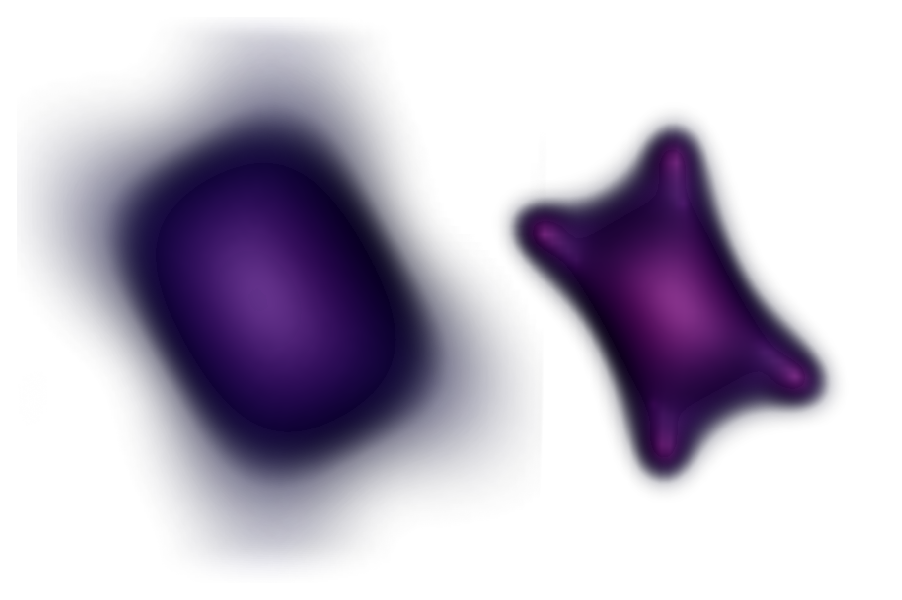
\includegraphics[scale=0.55]{Figures/pdf.eps}
\centering{}
\caption{Volumetric rendering of the diffusion propagator of a $60\,^{\circ}$ crossing with standard DSI(left) and DSI with deconvolution(right). \label{Fig:pdf}}
\end{figure}


\subsection{Q-ball Imaging}

Spherical harmonics (SH) are mathematical functions that can be used to
construct an orthonormal basis for a function on the sphere. In practice, these
can be used to approximate any spherical function (such as the ODF) up to a
highest frequency (SH order). Due to their practical mathematical properties,
there have been several cases of using spherical harmonics to describe dMRI
data, starting from the work of \citet{Frank2001, Frank2002} and
\citet{tuch-reese-etal:02}. In fact, Tuch showed that the Funk Radon Transform
(FRT), used in a method he called q-ball imaging (QBI), reconstructs a smoothed
version the ODF directly from a \emph{single spherical shell} dMRI
acquisition. This q-ball ODF $\psi_{QBI}$ can be obtained analytically from a
SH estimation of the diffusion signal \citep{descoteaux-angelino-etal:07,
  hess-mukherjee-etal:06, anderson:05}:
\begin{equation}\label{eq.qball}
\psi_{QBI}(\theta, \phi) = \sum_{j=1}^{R} 2\pi \frac{c_j}{S_0} P_{l(j)} (0) Y_{j} (\theta, \phi)
\end{equation}
where $P_{l(j)}$ is the Legendre polynomial of order $l$ corresponding to
coefficient $j$ and the coefficients have been normalized by the S0
image. Hence, the q-ball ODF is a linear transformation of the SH coefficient,
$c_j$. This technique is called analytical QBI (aQBI), in contrast to the
original QBI solution, which performs the FRT numerically.  The SH of order $l$
and phase $m$, $Y_{l}^{m}(\theta, \phi)$, arise from the angular solution to
Laplace's equation in spherical coordinates and they form an orthonormal basis
for complex functions defined on the unit sphere. However, in single-shell
acquisitions, S is real and symmetric. Hence, it is common to define a real and
symmetric modified orthonormal SH basis, $Y_{j}$, using only even order terms
and real/imaginary parts of $Y_{l}^{m}(\theta, \phi)$. Therefore, the measured
signal S is estimated with a truncated SH series of order $l_{max}$, which has
$R = (l_{max} +1)( l_{max} +2)/2$ terms. For example, for $l_{max} = 4, 6, 8$,
and $16$ SH series have $R = 15, 28, 45$, and $153$ coefficients respectively.

In Dipy we have implemented 3 different Q-ball methods in module
\texttt{dipy.reconst.shm}: a) \citep{descoteaux-angelino-etal:07}, b)
\citep{aganj-lenglet-etal:10} and c) \citep{tristan-vega-westin-etal:09}. For
example (a) can be used in the following way:
\begin{python}
from dipy.reconst.shm import QballModel
qb_model = QballModel(gtab, order=6, smooth=0.006)
qb_fit = qb_model.fit(data)
qb_odf = qb_fit.odf(sphere)
from dipy.reconst.odf import minmax_normalize
qb_nodf = minmax_normalize(qb_odf)
\end{python}
Important points here are that SH order needs to be $6$ and the regularization
parameter $0.006$. Furthermore, because the analytical ODF method produces more
rounded ODFs it is useful for visualization purposes to use min-max
normalization. The SH coefficients are accessible using the attribute
\texttt{qb\_fit.shm\_coeff}. Methods (b) and (c) can be used in a very similar
way. For example, for the Constant Solid Angle (CSA)
\citep{aganj-lenglet-etal:10} method (b) we only need to remove the
normalization function and reduce the SH order as the CSA method becomes
considerably noiser in higher orders:
\begin{python}
from dipy.reconst.shm import CsaOdfModel
csa_model = CsaOdfModel(gtab, order=4,
                        smooth=0.006)
csa_odf = csamodel.fit(data).odf(sphere)
\end{python}
On a side note the term Constant Solid Angle derives from the fact that this
method calculates the ODF with the radial distance in mind as we saw in
eq.~\ref{eq:ODF_DSI}. The analytical Q-ball method does not integrate the $r^2$
term and therefore it generates more rounded ODFs that require normalization.

\subsection{Constrained Spherical Deconvolution}

The method of spherical deconvolution \citep{tournier-calamante-etal:04} can be
used to estimate the distribution of fibre orientations present within each
voxel. With this method, the signal measured on single spherical shell
acquisitions can be expressed as the convolution over spherical coordinates of
the response function with the fiber orientation distribution. The response
function describes the signal intensity that would be measured as a function of
orientation for a single fiber aligned along the z-axis. In the spherical
harmonics (SH) framework, the convolution operation is performed as
follows. For each harmonic order $l$, the SH coefficients of the signal profile
$S(\theta, \phi)$ and the FOD $F(\theta, \phi)$ are written as vectors
$\mathbf{s}_l$ and $\mathbf{f}_l$ of length $2l+1$, whereas the rotational
harmonic coefficients of the convolution kernel R (the response function) are
written as a matrix $\mathbf{R}_l$ of size $(2l+ 1)\times(2l+ 1)$. The
convolution operation then simply consists of one matrix multiplication per
harmonic order l: $\mathbf{s}_l=\mathbf{R}\cdot\mathbf{f}_l$. The spherical
deconvolution operation can be performed by simple matrix inversion. However,
the spherical deconvolution problem is ill-posed and thus susceptible to noise.

Constrained super-resolved spherical deconvolution (CSD)
\citep{tournier-calamante-etal:07} gives a robust solution to this problem by
applying two major constraints on the fitting of the fODF. The first is that it
applies a non-negativity constraint: fODF values that are smaller than 0 are
non-physical and are precluded. The other is that CSD applies a sparseness
constraint on the fODF - it assumes that only a few of the fODF values will be
larger than 0. Applying these two constraints allows fitting the SH basis
up to very high orders - in essence fitting more parameters than data allow. 
This is known as \emph{super-resolution}. This super-resolved method
can be accessed in Dipy using:
\begin{python}
from dipy.reconst.csdeconv import
        ConstrainedSphericalDeconvModel as CsdModel
csd_model = CsdModel(gtab, response)
\end{python}
The main choice to be considered is the estimation of the single fiber response
function.  We assume that $R$ is derived from a prolate tensor. The eigenvalues
of this tensor are estimated from the voxels with FA $> 0.7$. The input
parameter \texttt{response} is a tuple with two parameters: a) the eigen-values
of the tensor and b) the estimated average S0 signal for those voxels. The
response function is usually estimated from the corpus callosum areas. For
further information on how to iniate the CSD please read our examples in
\texttt{dipy.org}.

Dipy also implements a second constrained spherical deconvolution method: The
Spherical Deconvolution Transform (SDT) is a sharpening operation which
transforms the smooth diffusion ODF into a sharper fiber ODF. The method is
inspired by CSD \cite{tournier-calamante-etal:07} with, the main difference
that the CSD is applied directly to the initial signal and the SDT directly to
the ODF \citep{descoteaux:08}.

The idea here is that an ODF, for example the analytical Q-ball ODF
$\psi_{QBI}$, can be formed by the convolution between the single fiber
diffusion ODF kernel $R$ and the true fiber ODF $\psi_{SDT}$.
\begin{equation}
\psi_{QBI}(\mathbf{u})=\displaystyle\int_{|w|=1} R(\mathbf{u} \cdot \mathbf{w}) \psi_{SDT}(\mathbf{w}) dw\label{eq:Conv}
\end{equation}
Therefore, the deconvolution of $\psi_{QBI}$ can recover a sharper
$\psi_{SDT}$. We can derive the formula for the $\psi_{SDT}$ using symmetrized
spherical harmonics.
\begin{equation}
\psi_{SDT}(\mathbf{u})=\displaystyle\sum_{j=1}^{R}2\pi P_{l_{j}}(0) \frac{c_j}{f_j}Y_{j}(\mathbf{u})\label{eq:ODF_SDT}
\end{equation}
For the derivation and explanation of the formula see \cite{descoteaux-deriche-etal:09}.
\begin{python}
from dipy.reconst.csdeconv import
        ConstrainedSDTModel as SdtModel
sdt_model = SdtModel(gtab, ratio)
\end{python}
Here the response function is provided as a scalar parameter, the ratio of the
smallest eigenvalue over the largest eigenvalue. Both spherical deconvolution
methods perform similarly \citep{GaryfallidisISBI2013a}.

In Fig.~\ref{Fig:ten_csa_csd} the ODFs of the \texttt{TensorModel}, \texttt{CsaOdfModel} and \texttt{CsdModel} in of a region in the centrum semiovale crossed by the splenium of the corpus callosum are shown. 

\begin{figure*}
\centerline{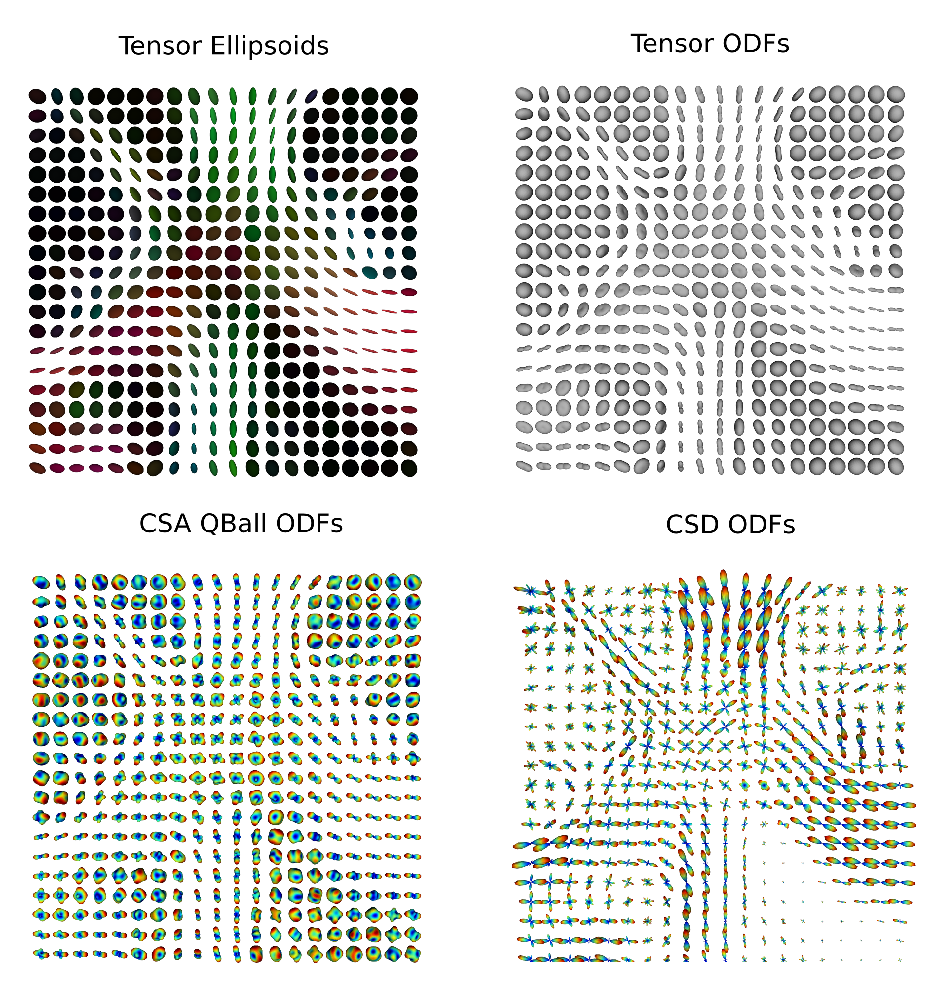
\includegraphics[width=180mm]{Figures/ten_csa_csd2.eps}}
\caption{a) Tensor ellipsoids color-coded with a DEC map, b) Tensor ODFs, c) Constant solid angle ODFs and d)super-resolved constrained spherical deconvolution ODFs\label{Fig:ten_csa_csd}}
\end{figure*}


\subsection{Peaks from models}
In the previous sections we showed that the reconstruction models have a
uniform API and can be called in similar ways. For example, they all have an
odf() method. This design gives us the opportunity to create utility functions
where the model is one of the parameters. \texttt{peaks\_from\_model} is a
multipurpose function which can be used to a) find the maxima (peaks) of the
ODFs, b) find the directions of the maxima in the ODFs which can be useful for
tracking, c) discretize those directions on the unit sphere for efficiency, d)
compress the ODFs as spherical harmonics to reduce memory usage and e)
calculate many metrics simultaneously, e.g. generalized fractional anisotropy
(GFA)[REF], without the need of creating all ODFs at
once. \texttt{peaks\_from\_model} can be called as:
\begin{python}
from dipy.reconst.odf import peaks_from_model
pmd = peaks_from_model(model=dsi_model,
                       data=data,
                       sphere=sphere,
                       relative_peak_threshold=.8,
                       min_separation_angle=45,
                       mask=mask,
                       return_odf=False,
                       return_sh=True)
gfa = pmd.gfa
\end{python}
The model parameter can be any of the models discussed in the previous sections
e.g. \texttt{dsi\_model}. The \texttt{relative\_peak\_threshold} parameter
enforces that only peaks greater than \texttt{relative\_peak\_threshold}$*m$
will be returned, where $m$ is the value of the largest
peak. \texttt{min\_separation\_angle} sets the threshold for the minimum
angular distance in degrees between two peaks. If the peaks are closer than
this threshold only the larger of the two is returned. This two parameters help
to get robust fiber directions when the ODFs are
noisy. \texttt{peaks\_from\_model} returns a \texttt{PeaksAndMetrics} object
which holds all the different output arrays, \texttt{peak\_values},
\texttt{peak\_indices}, \texttt{gfa} \citep{tuch:04}, \texttt{qa}
\citep{yeh-etal:10}, \texttt{odf} and \texttt{shm\_coeff}.

If the parameter \texttt{return\_sh} is set to True then the ODFs will be
represented by their SH expansion. This serves as a memory usage reduction
strategy as the SH coefficients need much less memory than the ODF represented
on the sphere. If we want to calculate the ODF back from the SH coefficients we
can use the function \texttt{sh\_to\_sf}:
\begin{python}
odf_sh = pmd.shm_coeff
from dipy.reconst.shm import sh_to_sf
odf = sh_to_sf(odf_sh, sphere, sh_order=8)
\end{python}

\section{Fiber tracking}\label{fiber_tracking}
\subsection{Deterministic}

\subsubsection{EuDX}
Euler Delta Crossings~\citep{Garyfallidis_thesis} is the first tracking
method that was implemented in Dipy. We created an algorithm that has many
similarities with the classical deterministic methods~\citep{Mori1999,
  conturo-lori-etal:99, basser-pajevic-etal:00} and with more recent ones as
those described in Descoteaux et al.~\citep{descoteaux-deriche-etal:09} and Yeh
et al.~\citep{yeh-etal:10}. Our concentration was to create a simple
deterministic algorithm which can be used with very different families of
reconstruction models, work well in crossing areas and be efficient so that it
can be used to quickly inspect the reconstruction results. EuDX is applied
usually in native space image coordinates and it assumes that the voxel
dimensions are equal in all three dimensions. If the provided data do not have
isotropic voxel size then a reslicing preprocessing step to isotropic is
required.

In order to create streamlines we need to provide initially one or more seed
points $s$. The points from where the streamlines will start growing. These can
be chosen randomly or we can specify them explicitly. However, these seed
points need to be constrained by the volume's dimensions. Every seed point
$\mathbf{p}_{0}$ becomes the starting point for the track propagation. For the
integration we solve for
$\mathbf{p}_{t}=\mathbf{p}_{0}+\int_{0}^{t}\mathbf{v}(\mathbf{p}(\mathbf{s}))d\mathbf{s}$
and we perform the integration numerically using Euler's method
\begin{equation}
\mathbf{p}_{n+1}=\mathbf{p}_{n}+\mathbf{v}(\mathbf{p}_{n})\Delta s\label{eq:euler}
\end{equation}
\noindent where $\Delta s$ is the propagation step size which should be at
least smaller than the voxel size and $\mathbf{v}$ is the propagation
direction. Furthermore, EuDX uses trilinear interpolation for the calculation
of the next direction integrating directional information from the surrounding
voxels.

The first parameter of EuDX can be an array of dimensions $X\times Y\times Z$
like FA or $X\times Y\times Z \times W$ like the ODF, or quantitative
anisotropy (QA)~\citep{yeh-etal:10}. These arrays can be used for stopping the
propagation if the value in the current voxel is lower than
\texttt{a\_low}. For efficiency, the peak directions are discretized on a unit
sphere. For this purpose, the second parameter is another array of dimensions
$X\times Y\times Z$ or $X\times Y\times Z\times W$ but this time these are the
indices of the directions approximated on the sphere. An example is given here
for tensor based streamlines:
\begin{python}
from dipy.tracking.eudx import EuDX
eu = EuDX(a=FA, ind=peak_indices, seeds=10**4,
          sphere=sphere, a_low=0.2)
tensor_streamlines = [line for line in eu]
\end{python}
The input parameter \texttt{seeds} can be given as an integer, this will
generate random seeds in the entire volume, or it can be given as $N\times 3$
array of seed points. This last explicit specification of seed points has the
advantage that it allows us to seed from specific ROIs or from the gray matter
- white matter boundary which has been shown to generate more robust tracking
results \citep{Cote2013tractometer}. The instance of EuDX returns back an
iterator. In every call of the iterator a new streamline is returned. This
technique allows to save directly streamlines in the disk without loading all
streamlines in memory. In Fig.~\ref{Fig:pretty_streamlines} we show a human 
brain streamlines, approximating the brain's white matter connections, generated 
from EuDX. 

\begin{figure}
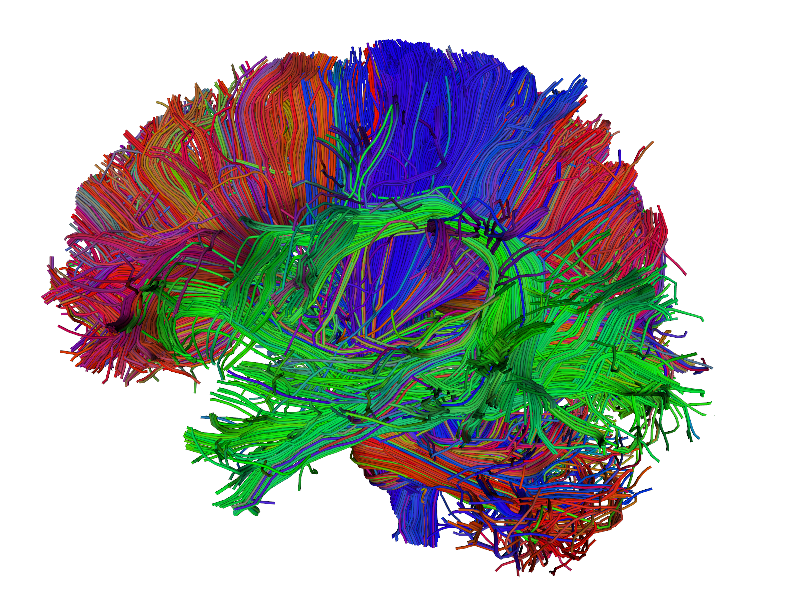
\includegraphics[scale=0.75]{Figures/pretty_streamlines.eps}
\centering{}
\caption{An example of EuDX-based fiber tracking applied on a real human brain dataset\label{Fig:pretty_streamlines}}
\end{figure}

\subsection{Probabilistic}

\section{Post-tracking}\label{post_tracking}

In the following sections we describe some of the tools available for processing
streamlines after these have been created.
\subsection{Streamline clustering}\label{quickbundles}
Depending on the initial number of seeds and other tracking parameters
fiber tracking algorithms can generate a great number of densely packed
streamlines (often more than one million) which is difficult to interact
and interpret. As a solution to this problem Dipy implements a recent and
efficient clustering algorithm for streamlines. This is called QuickBundles (QB)
[REF] and it can be used to simplify large datasets in a couple of minutes.
When using QuickBundles we need first to instantiate the object with 3
parameters. The first parameter is the set of initial streamlines to be
clustered, the second is the distance threshold that defines the cluster size
and the third is the level of detail for each streamline. For example, in the
the code snippet below we used \texttt{pts=18} which means that before QB
starts the clustering procedure the streamlines will be downsampled so that
each one has the same number of points (here 18) and equal segments. This
preprocessing step is a prerequisite for QB.
\begin{python}
from dipy.segment import QuickBundles
qb = QuickBundles(streamlines, dist_thr=20.,
                  pts=18)
\end{python}
After we have created the instance of the object, attributes like
\texttt{qb.centroids} provide the clusters' centroids and methods like
\texttt{qb.label2tracks()} can return the streamlines which belong to a
specific cluster.

\subsection{Counting streamlines in ROIs}

It is often useful in dMRI to find from which ROIs a streamline is passing
or even to count the number streamlines that go through an ROI [REF]. For this
purpose we created a multipurpose function called \texttt{track\_counts}.
\begin{python}
from dipy.tracking.vox2track import track_counts
tcs, tes = track_counts(streamlines,
                        volume_shape,
                        return_elements=True)
\end{python}
Given a set of streamlines and the shape of the 3D volume that the streamlines
were created we find whether a point of a streamline passed through a voxel by
rounding the mm point values to voxels. For a streamline that passes through a
voxel more than once, we only increase the count for the first point in
the streamline that enters the voxel. This information is returned in array
\texttt{tcs} of the same shape as \texttt{volume\_shape}. The entry
\texttt{tcs[i, j, k]} is the number of tracks that passed through voxel at voxel
coordinate i, j, k. If \texttt{return\_elements} is True we also return an object
array with one object per voxel. The objects at each voxel are a list of
integers, where the integers are the indices of the streamline that passed through
the voxel.

This function can be used to filter streamlines which go through specific masks,
calculate track densities [REF] or used for connectivity analysis.

\subsection{Streamline metrics and statistics}

In Dipy we have implemented a plurality of metrics for streamlines. For example,
perhaps the simplest thing that someone may want to do is to calculate the
average length and standard deviation of the streamlines generated after the
fiber tracking procedure. This can happen very easily using the \texttt{length}
function which takes as input a single streamline. We can then iterate through
all the streamlines in the following way:
\begin{python}
import numpy as np
from dipy.tracking.metrics import length
lengths = [length(s) for s in streamlines]
lengths = np.array(lenghts)
average_length = lengths.mean()
standard_deviation_lengths = lengths.std()
\end{python}
Many other metrics can be found in the metrics sub-module e.g. \texttt{spline} for
spline interpolation, \texttt{centre\_of\_mass}, \texttt{mean\_curvature},
\texttt{mean\_orientation} and the \texttt{frenet serret} framework for curvature
and torsion calculations along a streamline.

\subsection{Visualization}
Fig.~\ref{Fig:pdf},~\ref{Fig:ten_csa_csd},~\ref{Fig:pretty_streamlines} are generated by 
our own visualization tools which can be used for most parts of the diffusion 
analysis pipeline. We have developed a minimal, lightweight and up to the point 
module which is based on the Visualization Toolkit (VTK)[REF] and we call 
\texttt{fvtk}. The main idea is that window can have one or more renderers. 
A renderer can have none, one or more actors. Examples of actors are a sphere, 
line, point or a complete set of streamlines. You can basically add actors in a 
renderer and in that way you can visualize the forementioned objects e.g. 
sphere, line etc. The windows can
be created by either the \texttt{show} function which creates a visible window
or the \texttt{record} function which creates a temporary window only for the
purpose of using it to render the objects and save the frames on disk. The
renderer holds all the actors i.e. the visible objects. Here is a simple example
where we visualize some streamlines with different colors:
\begin{python}
from dipy.viz import fvtk
renderer = fvtk.ren()
line_actor = fvtk.pretty_line(streamlines,
                              streamline_colors)
fvtk.add(renderer, line_actor)
fvtk.show(renderer)
\end{python}
The most commonly used visualization functions are given in Tab.~\ref{fvtk_table}.

\begin{table}[th] \processtable{List of visualization functions\label{fvtk_table}}
{\begin{tabular}{rr} \hline
Name & Usage \\ \hline
ren & create renderer\\
add & add actor to renderer\\
rm  & remove actor from renderer \\
rm\_all & remove all actors from renderer \\
show & create window and show renderer \\
record & save frame or frames \\
line & actor of one or more streamlines \\
pretty\_line & same as line but with streamtubes \\
point & actor points as small spheres \\
tensor & actor of tensor ellipsoids \\
sphere\_funcs & actor for ODF visualization \\
volume & 3D volume rendering with raycasting \\
\hline
\end{tabular}}{}
\end{table}

\section{Discussion/Conclusion}

We have described the Dipy library for analysis of diffusion MRI data. Dipy is
a part of the Neuroimaging in Python community (\url{nipy.org}), a growing
community of scientists and developers who are participating in the development
of open source software for neuroimaging written in the Python language. 
Extend...

\section*{Acknowledgments}
One major source of support for this community comes in the form of the Neurodebian
distribution \citep{Halchenko2012}. Neurodebian is a platform for maintenance
and deployment of software for the analysis of neuroscience data, based on free
open source software (FOSS) practices.

Ariel Rokem is funded by a National Research Service Award (NEI F32 EY022294).
Eleftherios Garyfallidis if funded by ...

\section*{Disclosure/Conflict-of-Interest Statement}
There are no conflicts of interest.

% \section{LaTex Formatting}

% This is information for the coauthors of this paper. This section will be removed from the last version of this paper.

% This is to show how graphics (EPS) files are included. We use EPS for
% speed. The first one is spread across both columns, and the second one
% is just in a single column:

% \begin{figure*}
% \centerline{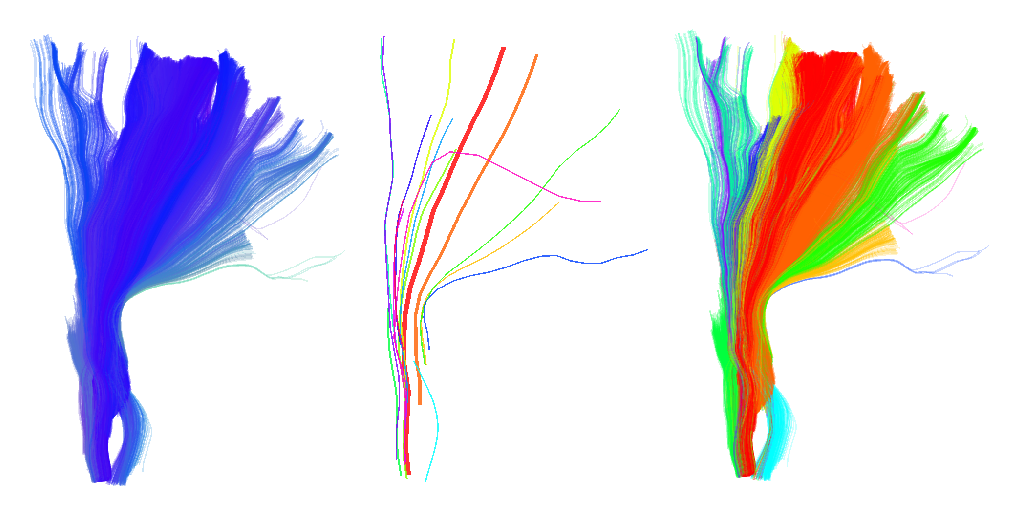
\includegraphics[width=160mm]{Figures/Fig_4_cst_simplification_relabeled_triple.eps}}
% \caption{This is the figure caption - and a label to refer to it in the text \label{Fig:big_picture}}
% \end{figure*}

% When we want to refer to this figure we use the label (see Fig.~\ref{Fig:big_picture}).

% \begin{figure}
% 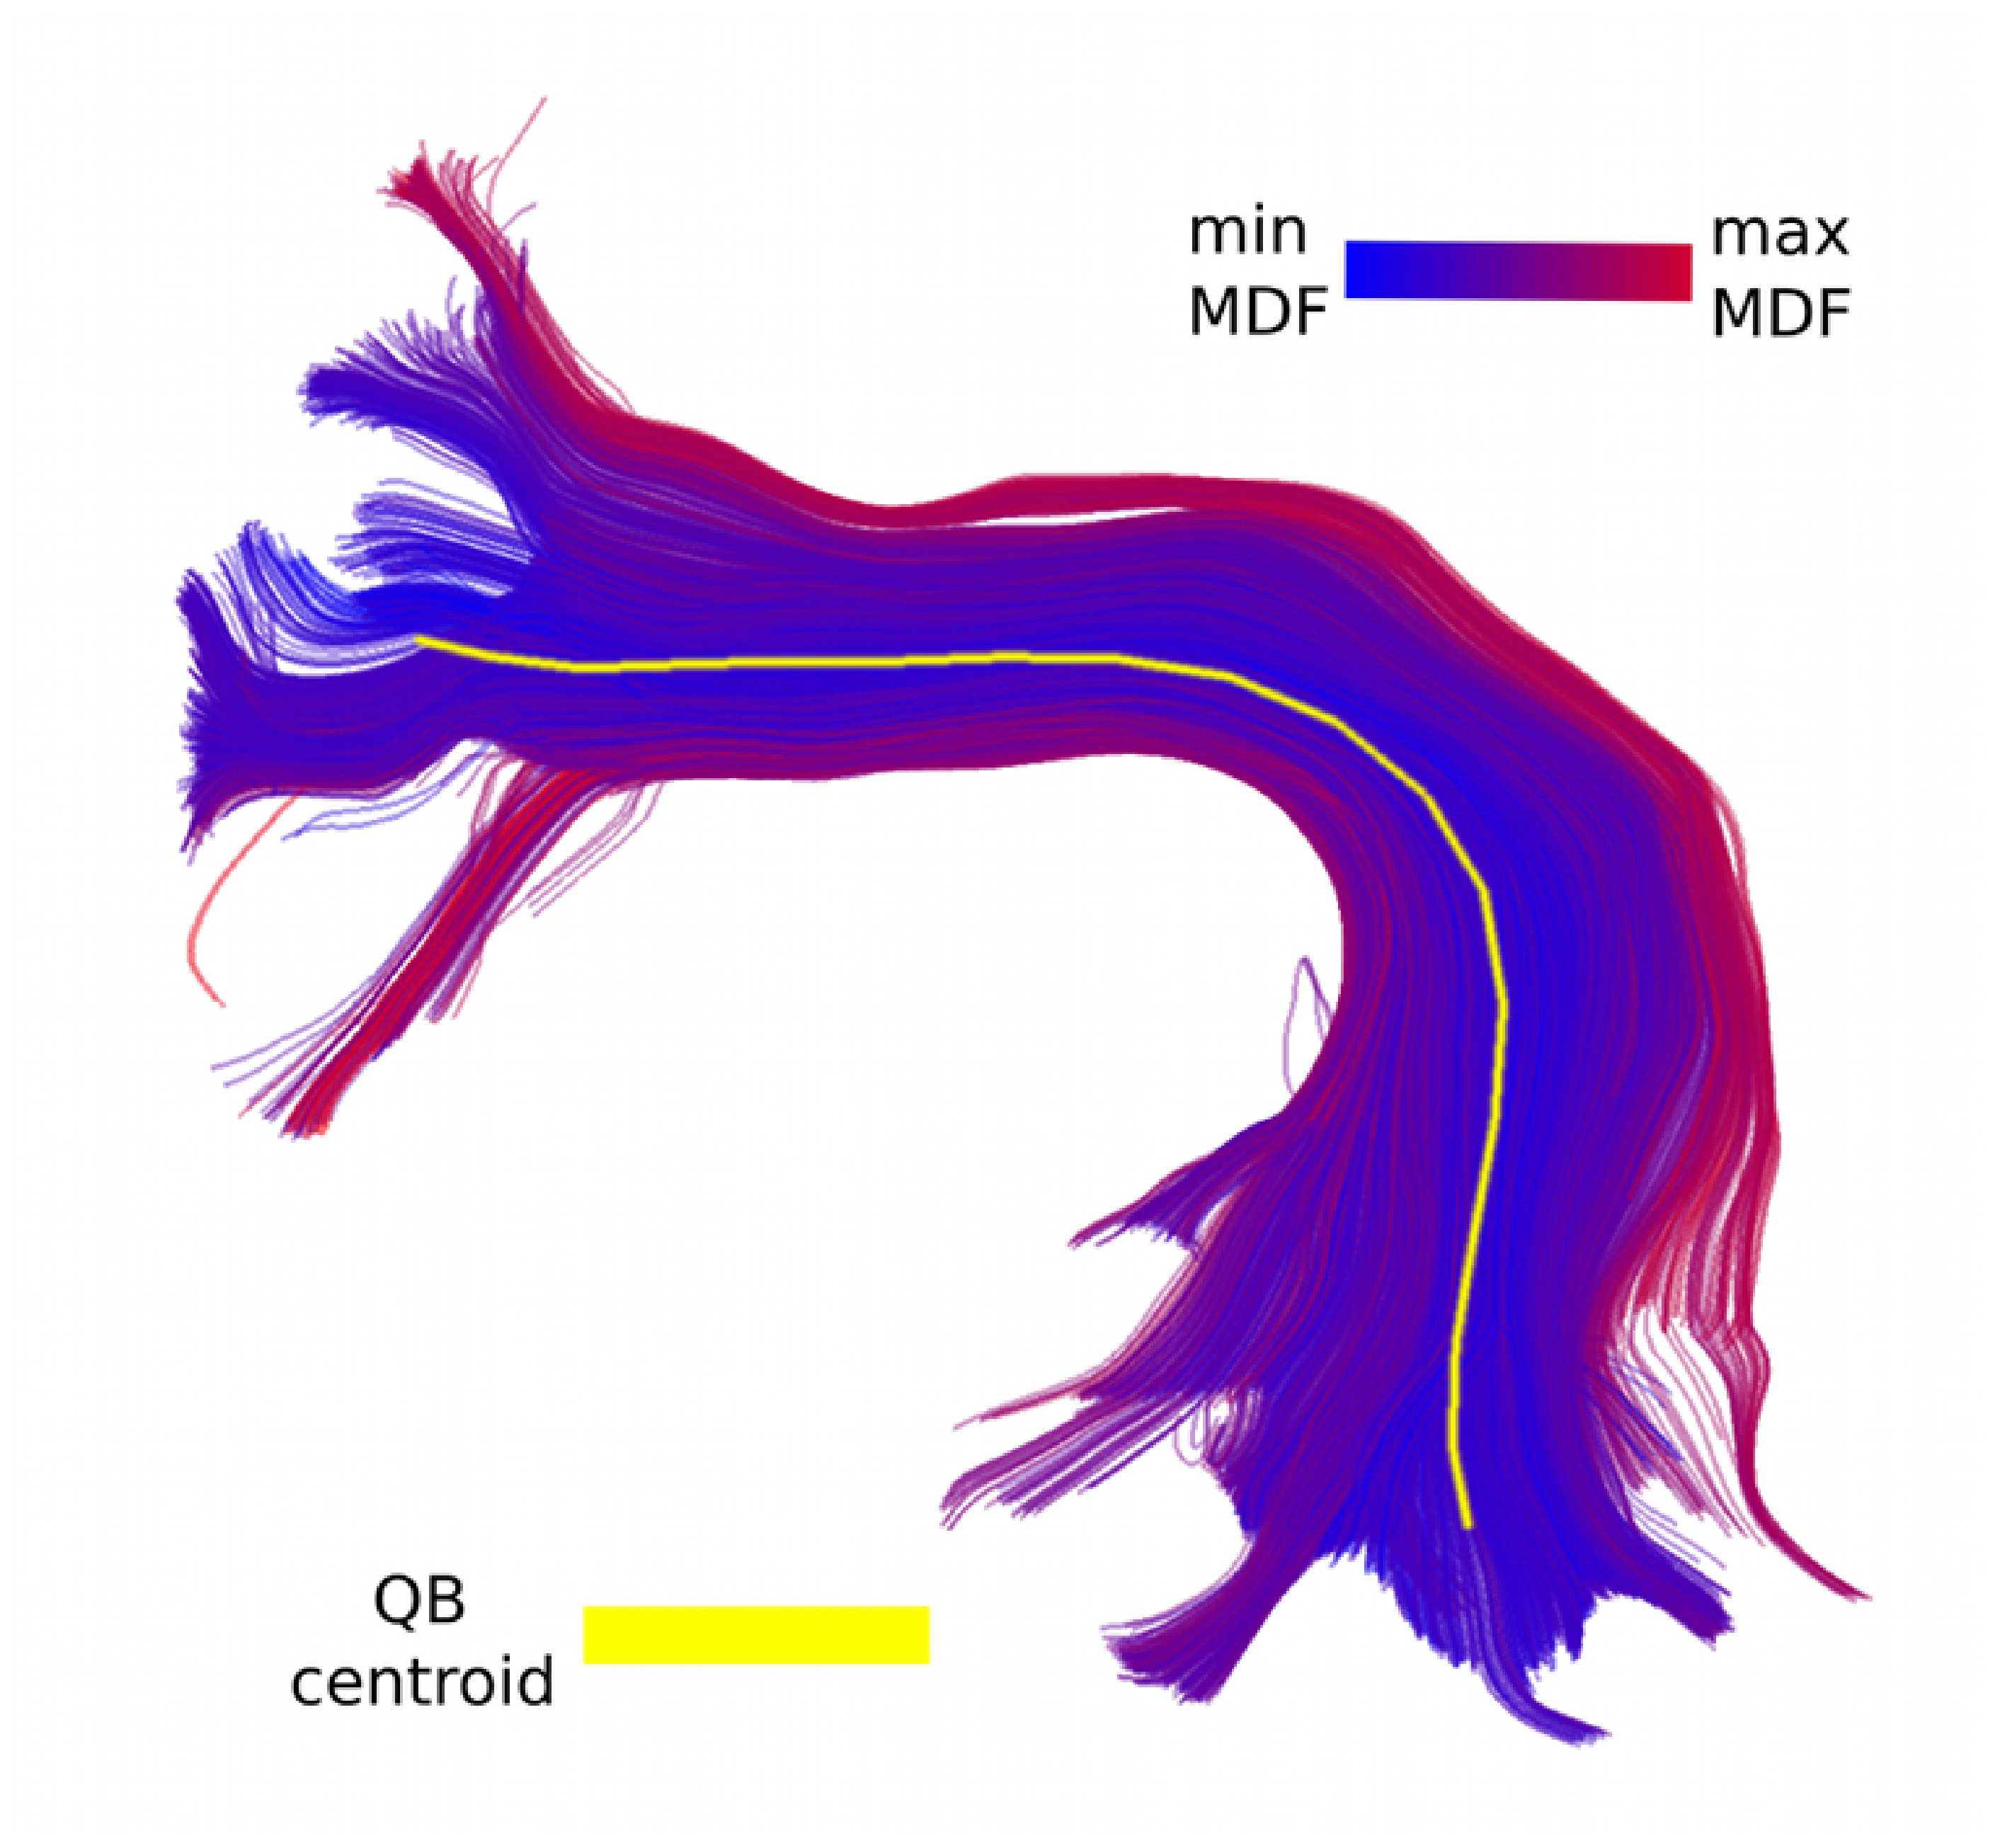
\includegraphics[scale=0.15]{Figures/Fig_11_MDF_arcuate}
% \centering{}
% \caption{Color coding shows MDF distances from QB centroid to every
%   other track in the bundle.\label{Fig:little_picture}}
% \end{figure}

% Here are some displayed equations (see Eq.~\ref{eq:direct_flip_distance}):
% \begin{eqnarray}
%   d_{\textrm{direct}}(s, t) = d(s, t) & = & \frac{1}{K}\sum_{i=1}^{K}|s_{i}-t_{i}|,\nonumber\\
%   d_{\textrm{flipped}}(s, t) & = & d(s,t^F) = d(s^F,t),\nonumber\\
%   \textrm{MDF}(s, t) & = & \min(d_{\textrm{direct}}(s, t), d_{\textrm{flipped}}(s, t))\label{eq:direct_flip_distance}.
% \end{eqnarray}

% Inline mathematics goes like this: $\frac{1}{K}\sum_{i=1}^{K}|s_{i}-t_{i}|$

% Here we have an example of a table (see Table~\ref{Table_1}).

% \begin{table}[th] \processtable{QB centroids performance compared with
% random subsets\label{Table_1}} {\begin{tabular}{rrrr} %\hline Thresholds &
% Comparison & Coverage \% (s.d.) & Overlap (s.d.) \\ \hline
% \multirow{2}{*}{$10$~mm/$10$~mm} & QB Centroids & 99.96 (0.007) & 2.44
% (0.08)\\ & Random & 90.49 (0.41) & 6.16 (0.55)\\ \hline
% \multirow{2}{*}{$20$~mm/$20$~mm} & QB Centroids & 99.99 (0.004) & 3.54
% (0.18)\\ & Random & 95.86 (0.62) & 6.81 (0.93)\\ \hline
% \end{tabular}}{}
% \end{table}

% References go like this: in parentheses \citep{Garyfallidis_thesis, Mori1999}, and in running text \citet{Garyfallidis_thesis}.

% And here is an example of how to add some code.

% \begin{python}
% from dipy.viz import fvtk
% ren = fvtk.ren()
% class Test(object):
%   def __init__(self, a):
%     pass
% @parametric
% def f(x):
%   return x**2
% for i in range(10):
%   print f(i)
% \end{python}


\selectlanguage{british}%
\bibliographystyle{apalike2}
%\bibliographystyle{plainnat}
%\bibliographystyle{IEEEabrv, IEEEtran}
%\bibliographystyle{IEEEtran}
%\bibliographystyle{elsarticle-harv}
\selectlanguage{english}
\bibliography{scilBibTex}

\end{document}
